\chapter{Frontend}
Bei dem Frontend handelt es sich um den in Java programmierten Client und Server.
Mit Ausnahme der Dateisynchronisation arbeitet es völlig unabhängig vom Backend.
Im Großen und Ganzen werden folgende Aufgaben erfüllt:
\begin{itemize}
	\item Netzwerkkommunikation zwischen den Clients und dem Archivserver.
	\item Programmierschnittstelle für Java-Tools, die das Archiv nutzen wollen.
	\item Benachrichtigung der Nutzer über Änderungen.
\end{itemize}
\section{Use-Cases}
In Use-Case Diagramm \ref{dia:design:frontend::usecase} sind alle wesentlichen Ereignisse (Use-Cases) zusammengefasst, die sich im Frontend abspielen.
\subsection{Update-Notifier} \ref{req:Sv:notifier}
Der Notifier arbeitet als eigenständiger Thread im Server.
\begin{description}
	\item [select] 
		\ref{req:Sv:comm:changes}
		Der Notifier führt in bestimmten Intervallen (\ref{req:Sv:notifier:interval})eigenständig Datenbankabfragen durch,
		um Änderungen zu ermitteln.
	\item [notifyClients und notifyObservers] \ref{req:Sv:notifier:notify},
		\ref{req:Cl:notifies}
		Die Änderungen werden an alle registrierten Clients gesendet.
		Die Clients wiederum geben die Änderungen an angemeldete Observer weiter.
\end{description}

\subsection{Java User} \label{design:frontend:usecase:user}
Java User stellen alle Akteure dar die den Client in ihr Programm einbinden. 

\begin{description}
	\item [initClient und registerClient]
		\ref{req:Cl:register}, \ref{req:Sv:register}
		beim starten des Client meldet sich dieser beim Server und wird dort registriert.
		Beendet sich ein Client so wird er aus der Registrierung genommen \ref{req:Sv:rmClients}
	\item [select]
		\ref{req:Cl:dbquery}, \ref{req:Sv:comm:dbquery}
		über vorbereite sql-select Schnittstellen können MetaDatenobjekte aus der
		Datenbank abgefragt werden.
	\item [getFileList]
		\ref{req:Cl:ls}, 
		Es wird eine Dateiliste eines \arc-Verzeichnisses zurückgegeben.
	\item [getOutputStream]
		\ref{req:Cl:writeFile}
		Es wird ein Outputstream zurückgegeben um Dateien in das Archiv zu schreiben.
	\item [getInputStream]
		\ref{req:Cl:readFile}
		Über einen Inputstream können aus dem Archiv gelesen werden.
	\item [getXMLData]
		\ref{req:Cl:selectTag}
		Es werden bestimmte XML-Daten zurückgegeben.
	\item [addXMLData]
		\ref{req:Cl:addTag}
		Es können neue Elemente zu den XML-Daten hinzugefügt werden.
	\item [add / deleteObserver]
		Es können Observer an- und abgemeldet werden, welche Update-daten aus dem
		Archiv bekommen können.
\end{description}
\begin{figure}[!h]
	\centering
	\label{dia:design:frontend:usecase}
	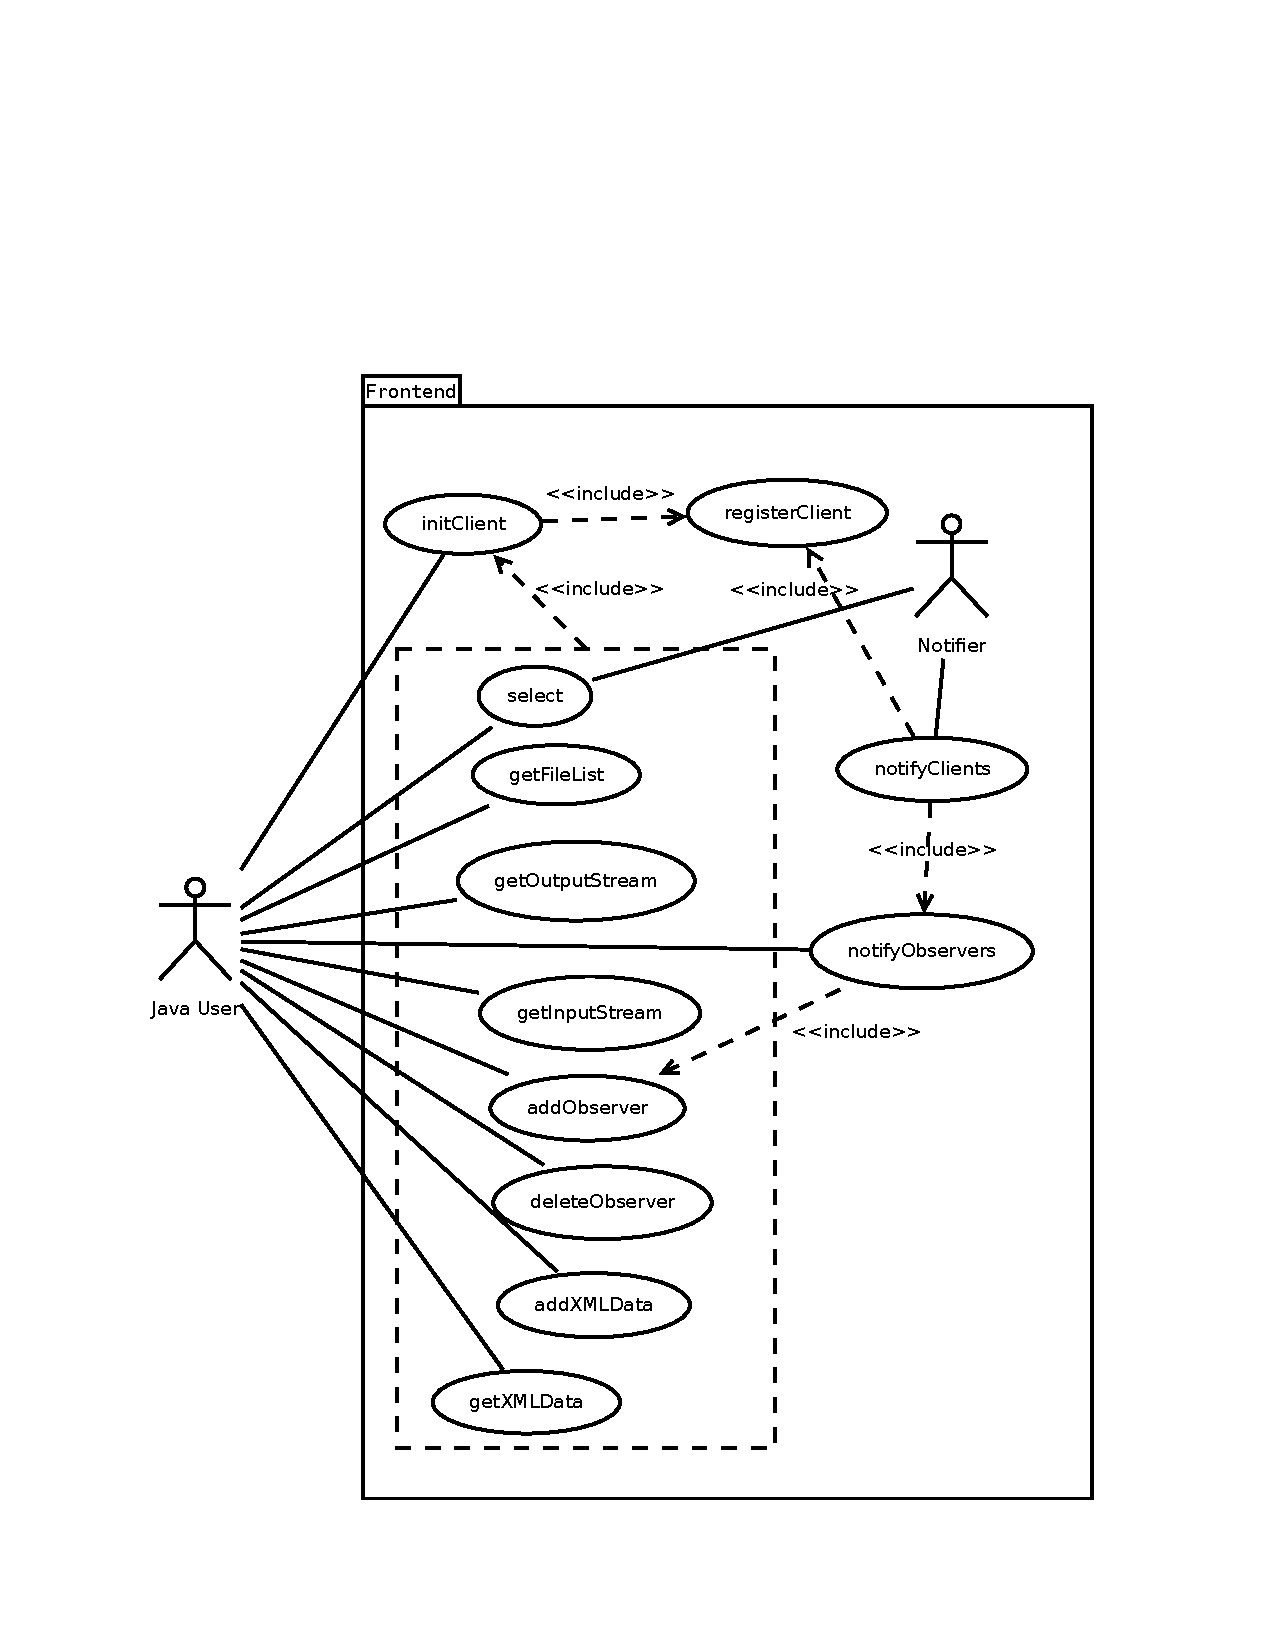
\includegraphics[height=0.9\textheight]{design/frontend/usecase.pdf}
	\caption{Diagramm: Use-Cases - Client und Server}
\end{figure}

\newpage

\section{API}
Neben den in Abschnitt \ref{design:data:classes} beschriebenen Datenklassen enthält die
API noch folgende Klassen und Interfaces:
\begin{description}
	\item [WebarchiveClientFactory]
		Die Factory bietet Möglichkeiten zur Konfiguration und Erzeugung der Clients
	\item [WebarchiveClient]
		Der WebarchiveClient ist die Zentrale Programmierschnittstelle an das Webarchiv.
		Es lassen sich Aktionen wie unter Abschnitt \ref{design:frontend:usecase:user} ausführen.
	\item [XmlEdit]
		Hilfsklasse zum Bearbeiten der XML-Dateien.
	\item [WebarchiveObserver]
		Implementierer dieser Schnittstelle werden über Updates benachrichtigt.
\end{description}
Details zeigt Diagramm \ref{dia:design:frontend:cl:api}
\begin{figure}[!h]
	\centering
	\label{dia:design:frontend:cl:api}
	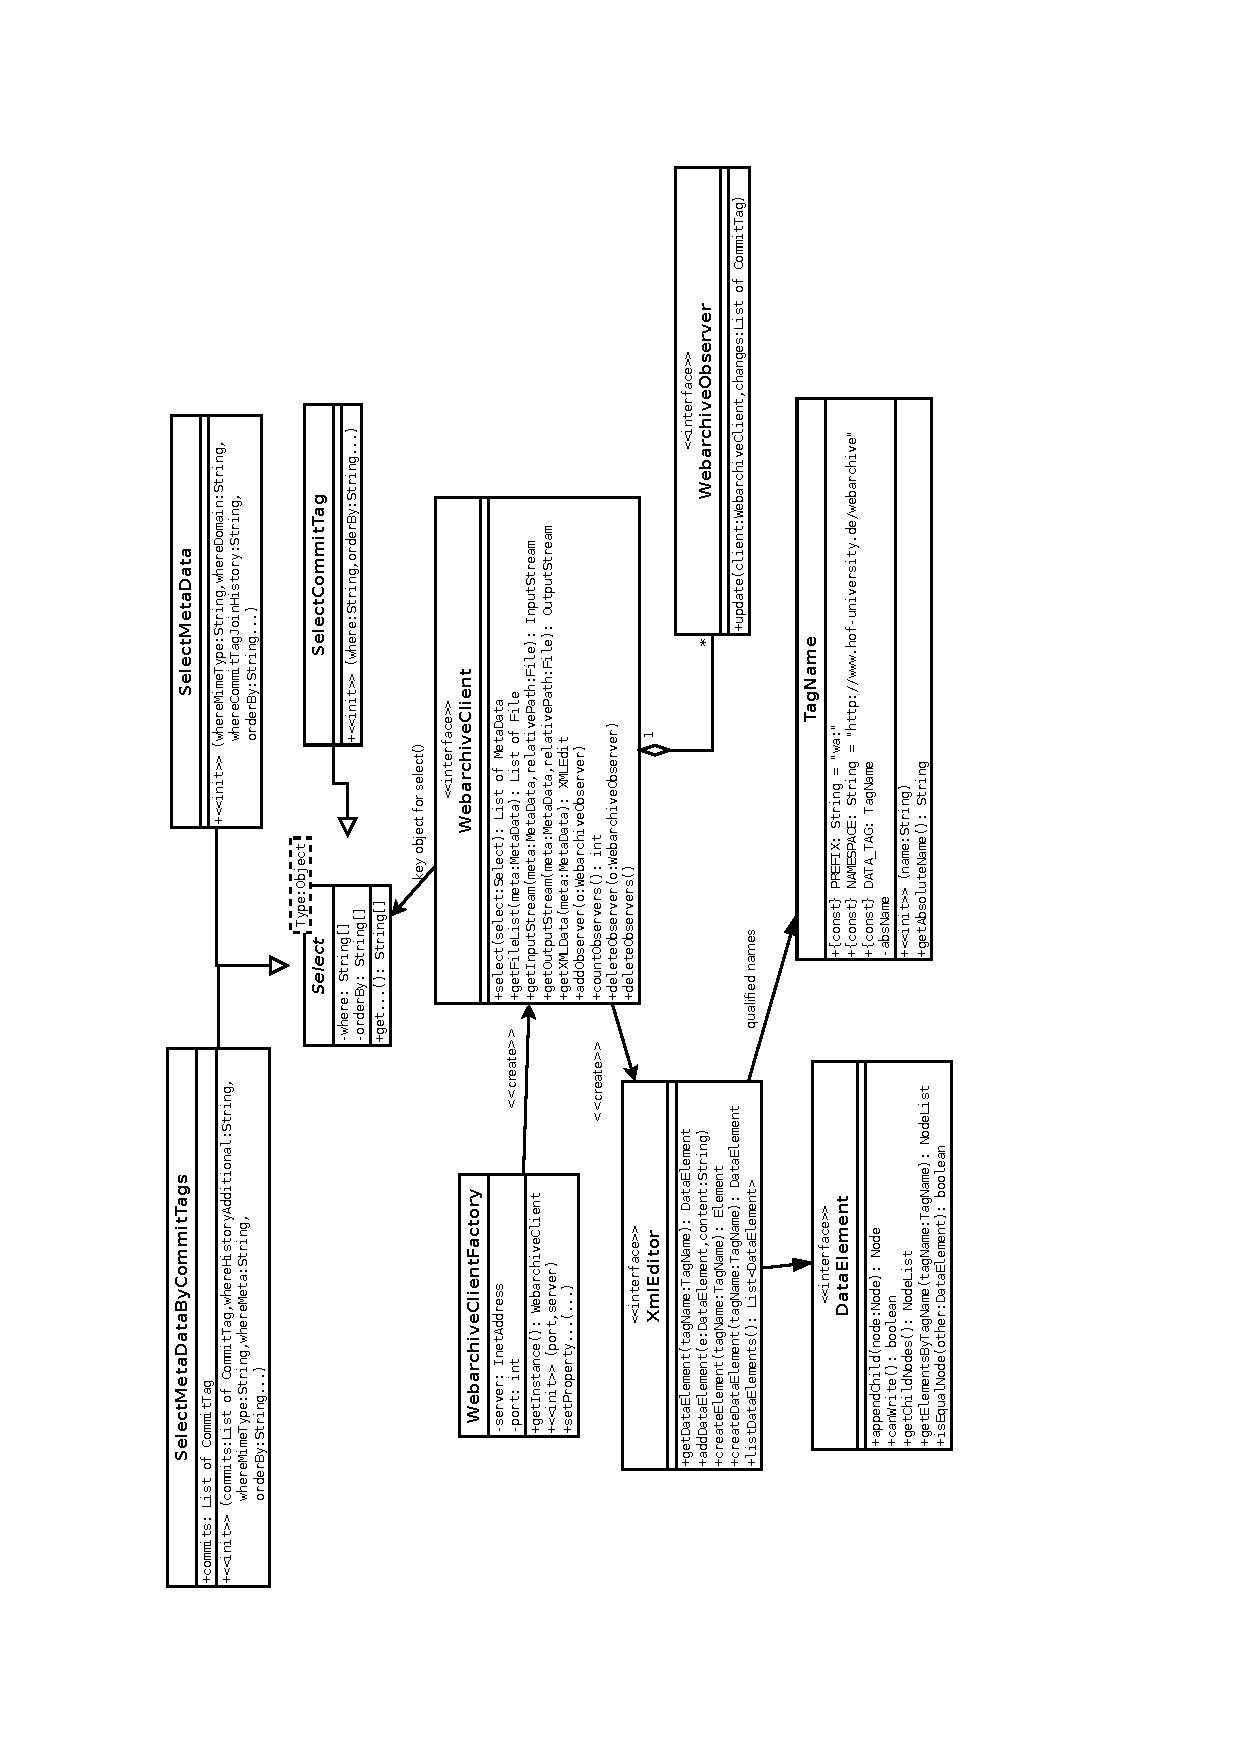
\includegraphics[angle=270, width=\textwidth]{design/frontend/classes/api-Klassen.pdf}
	\caption{Klassendiagramm: API}
\end{figure}

\section{Programmfluss}

\subsection {select}

\begin{figure}[h]
	\centering
	\label{dia:design:frontend:sqc:select}
	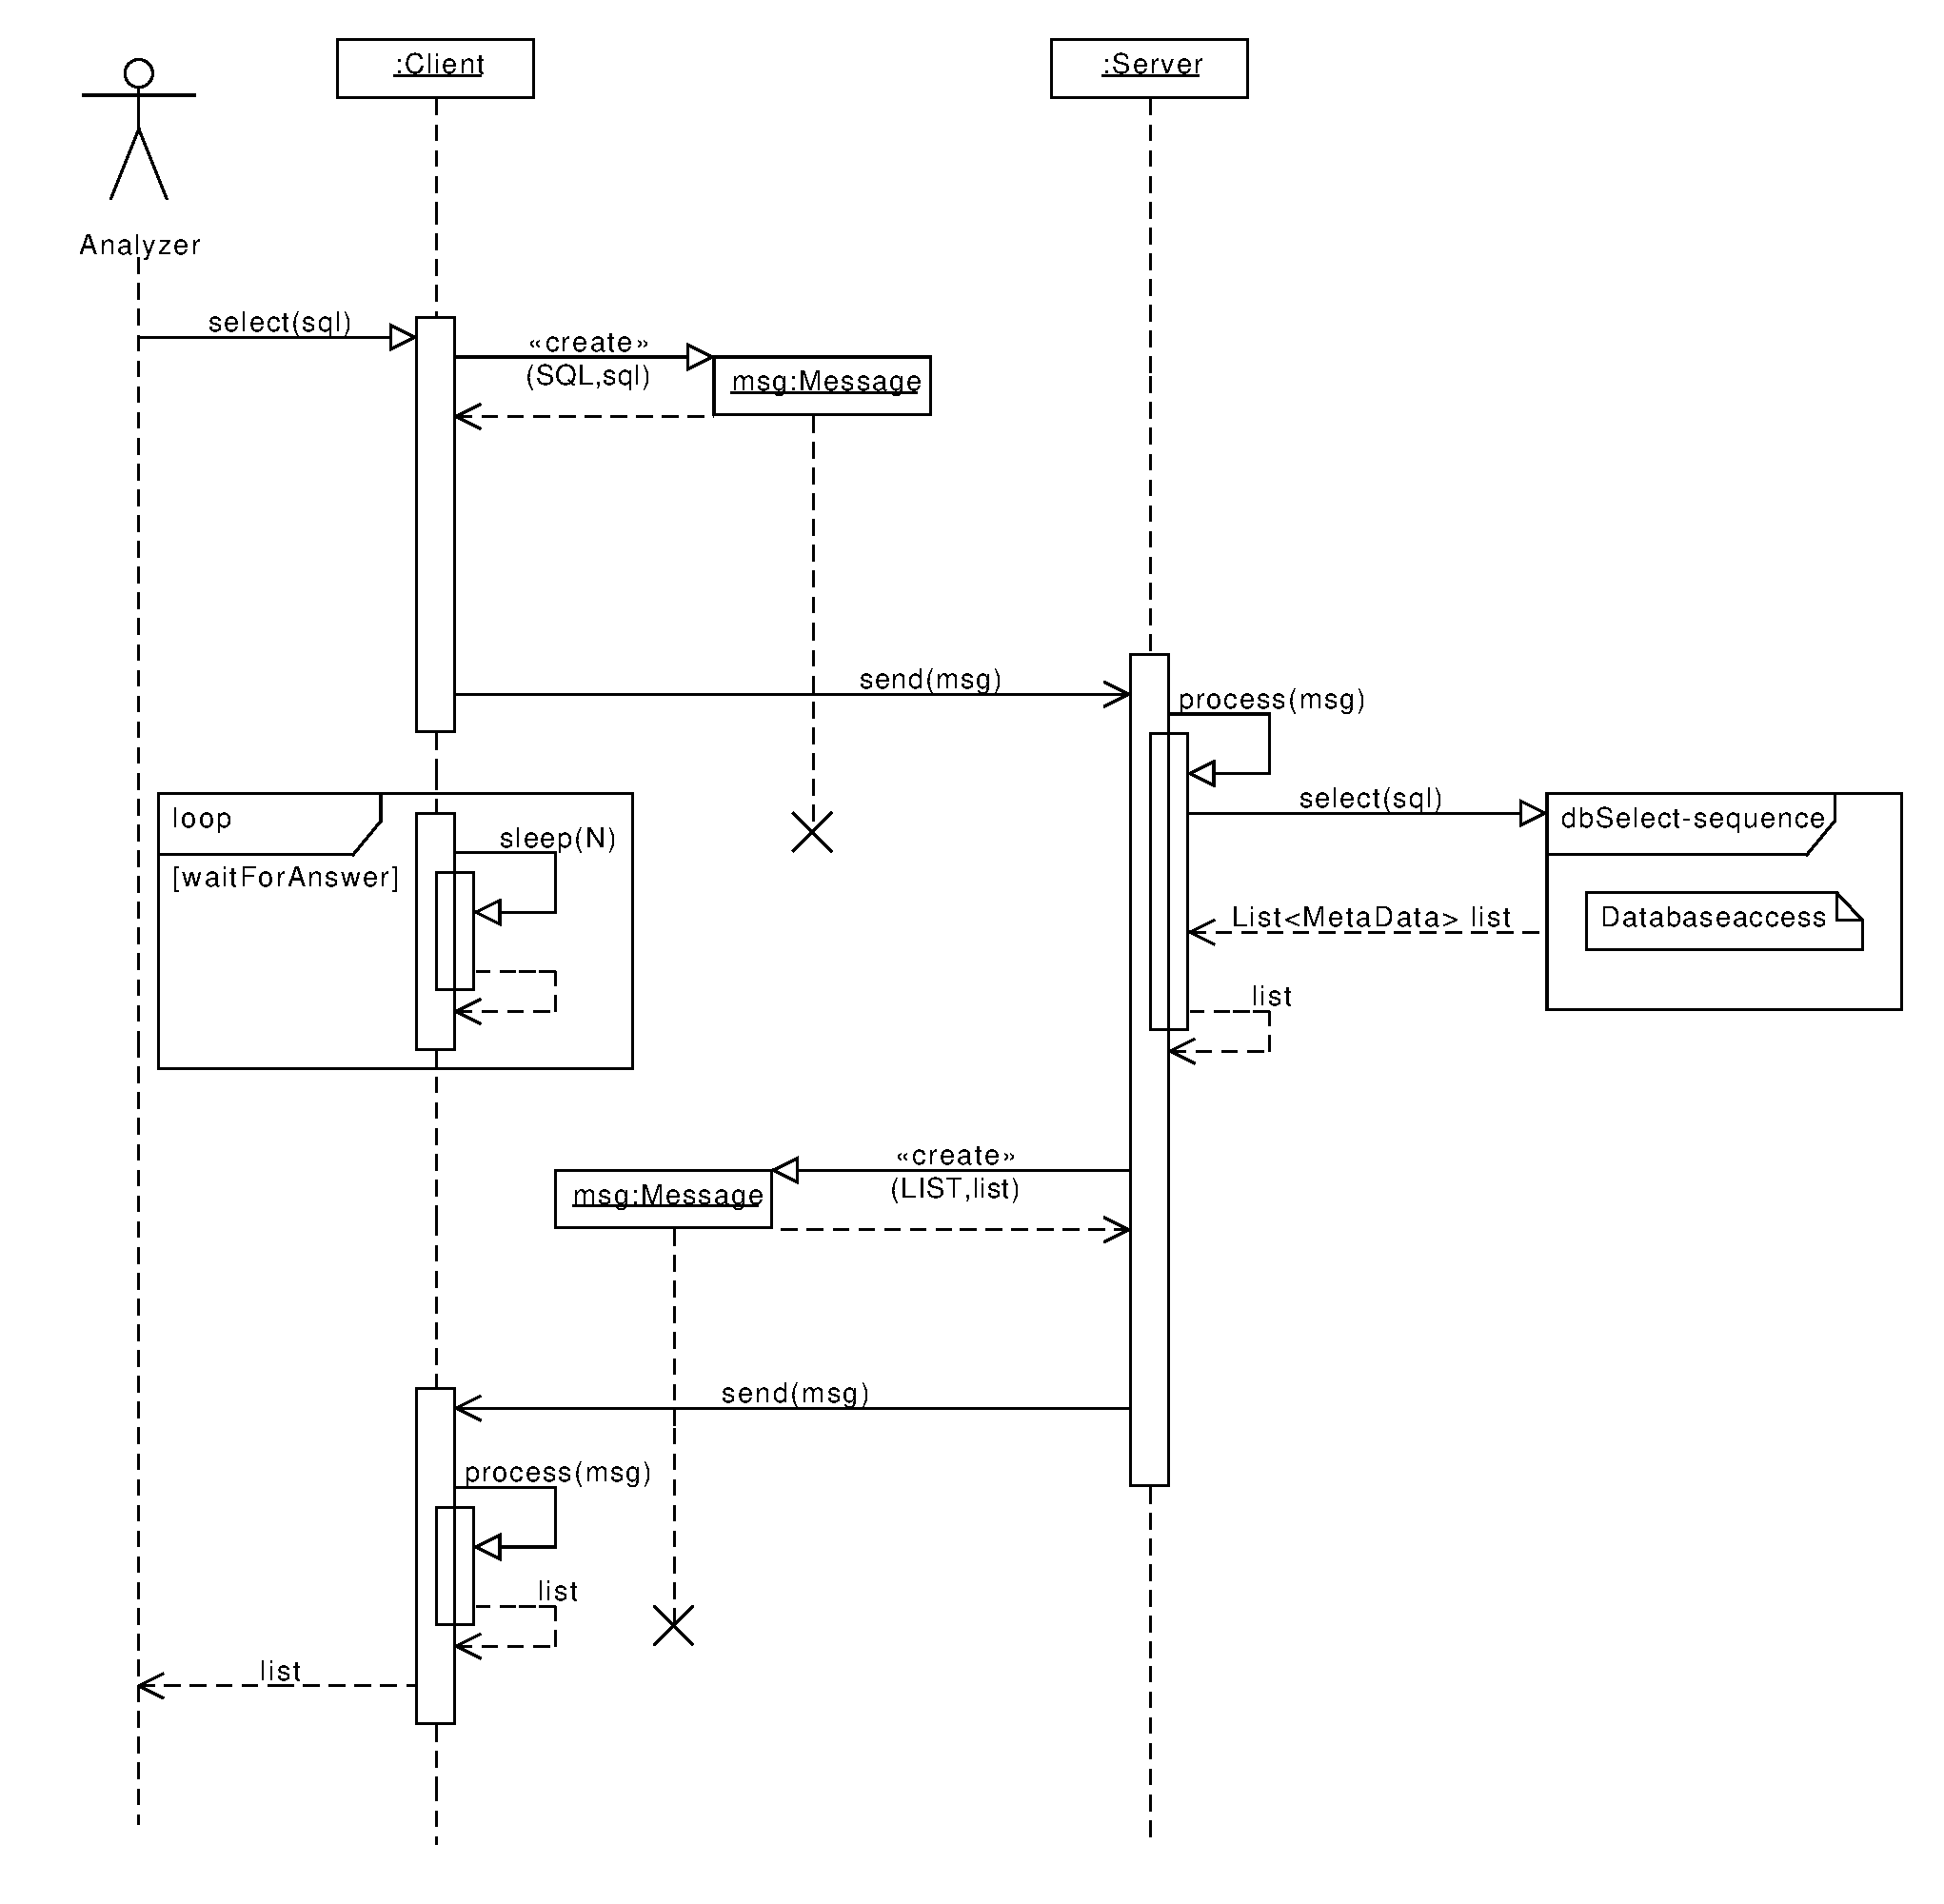
\includegraphics[width=\textwidth]{design/frontend/sequence/select-sequence.pdf}
	\caption{Sequenzdiagramm: Select}
\end{figure}

\subsection {getFileList}
\todo{sequence: getFileList}
%\begin{figure}[h]
%	\centering
%	\label{dia:design:frontend:sqc:select}
%	\includegraphics[width=\textwidth]{design/frontend/sequence/.pdf}
%	\caption{Sequenzdiagramm: Select}
%\end{figure}

\subsubsection{Lock setzen}
\begin{figure}[h]
	\centering
	\label{dia:design:frontend:sqc:lock}
	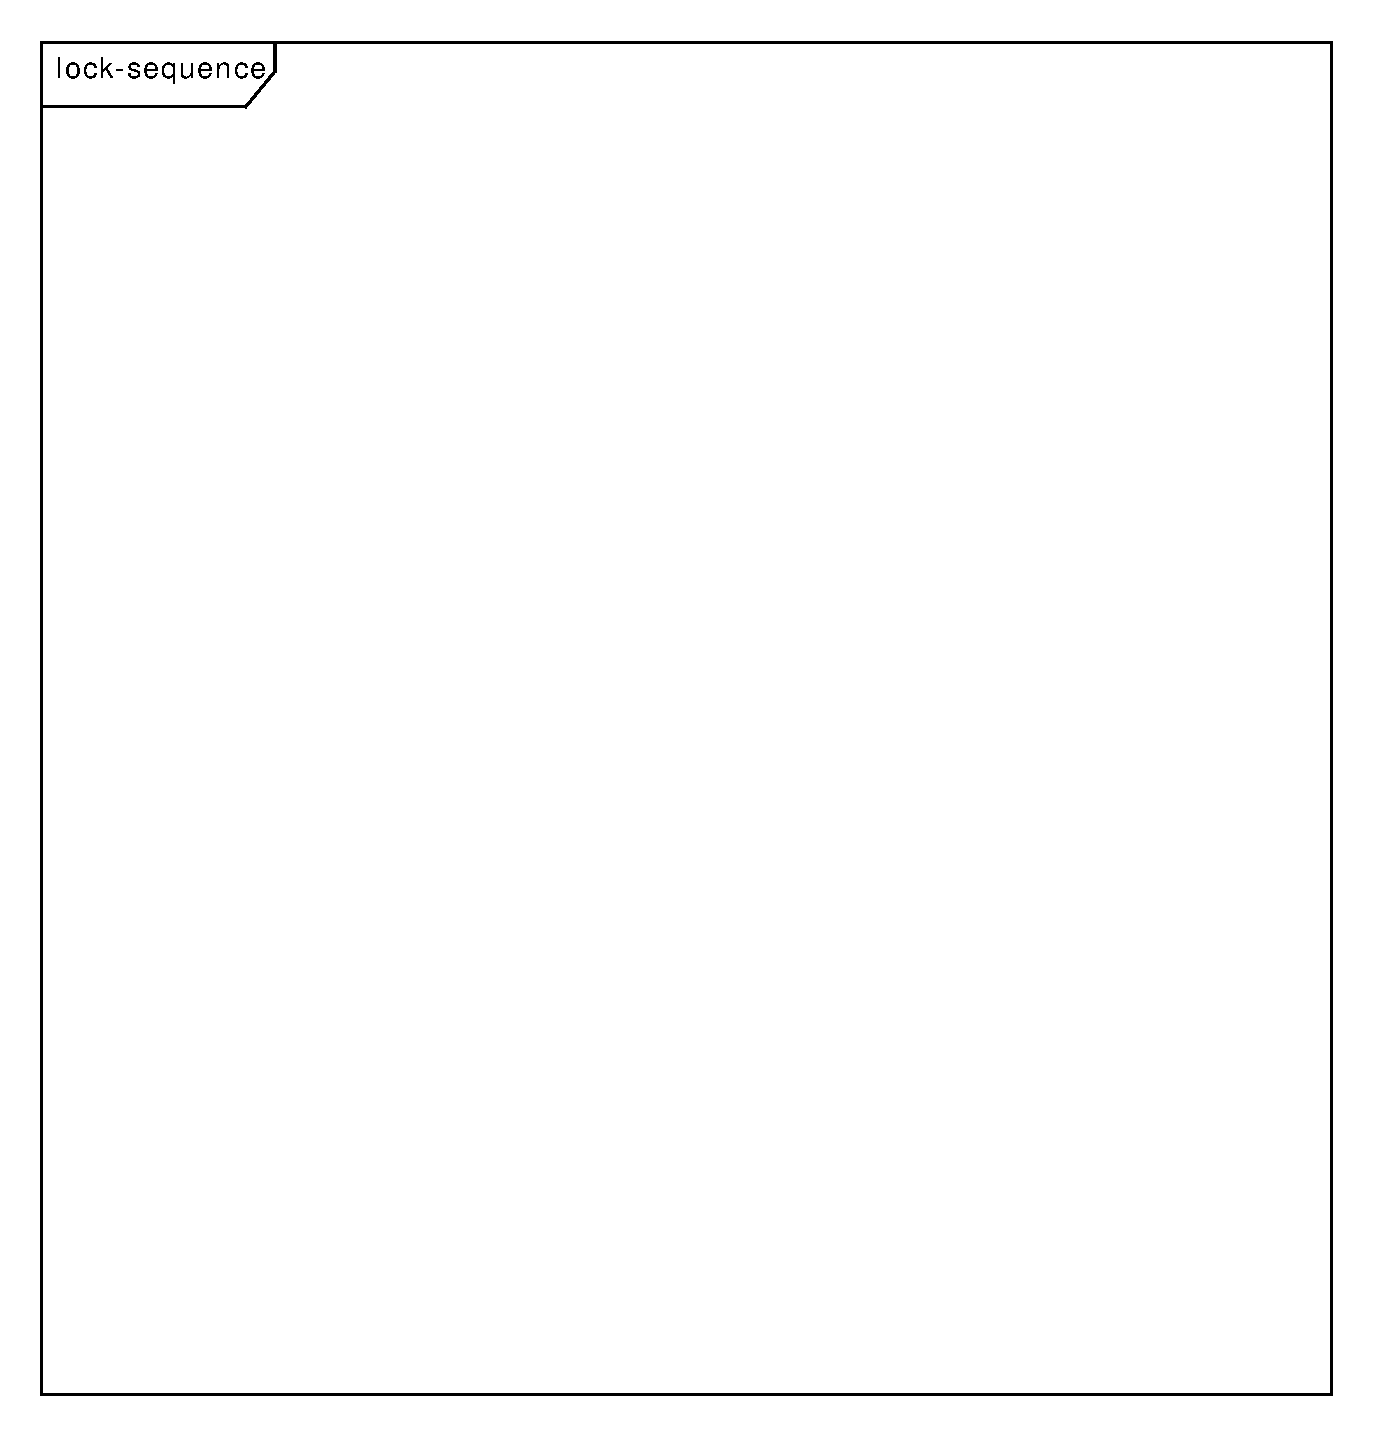
\includegraphics[width=0.5\textwidth]{design/frontend/sequence/lock-sequence.pdf}
	\caption{Sequenzdiagramm: Lock setzen}
\end{figure}

\subsubsection{Unlock}
\begin{figure}[h]
	\centering
	\label{dia:design:frontend:sqc:unlock}
	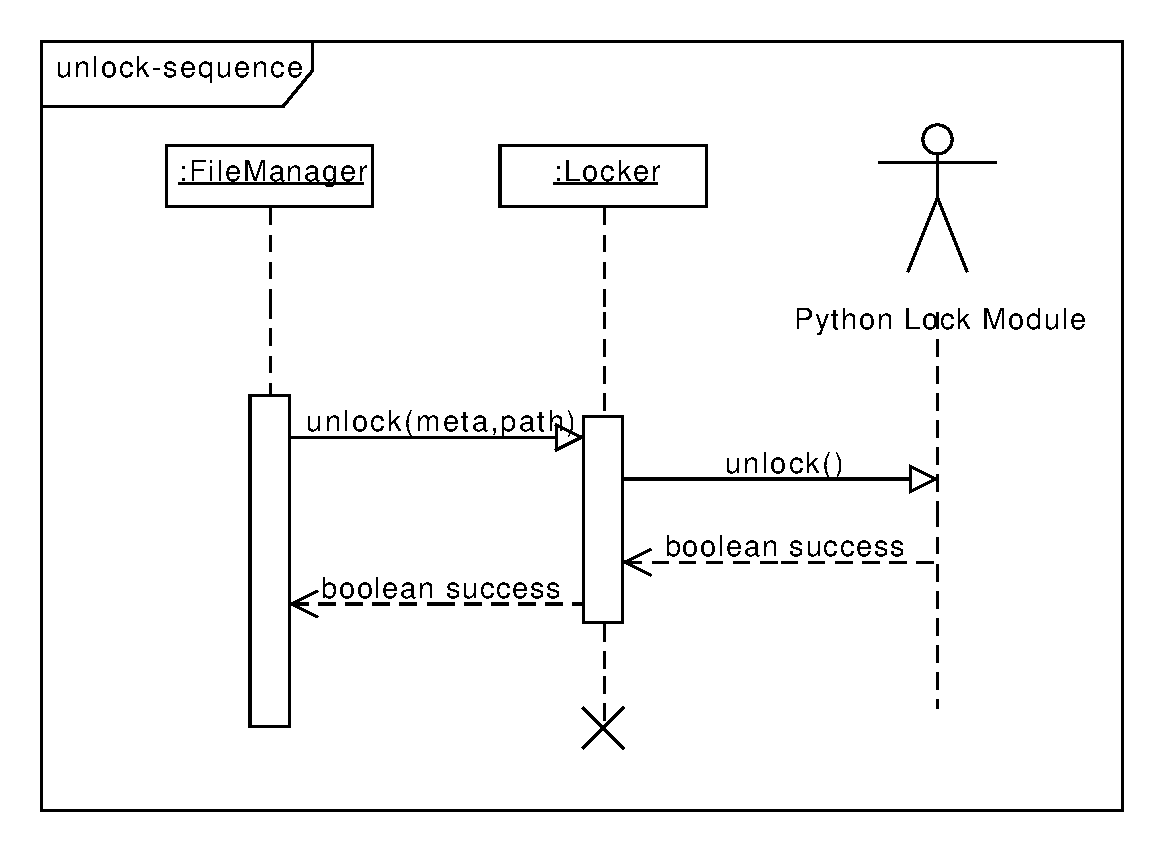
\includegraphics[width=0.5\textwidth]{design/frontend/sequence/unlock-sequence.pdf}
	\caption{Sequenzdiagramm: Unlock}
\end{figure}

\subsection {getOutputStream}
\begin{figure}[h]
	\centering
	\label{dia:design:frontend:sqc:getOutputStream}
	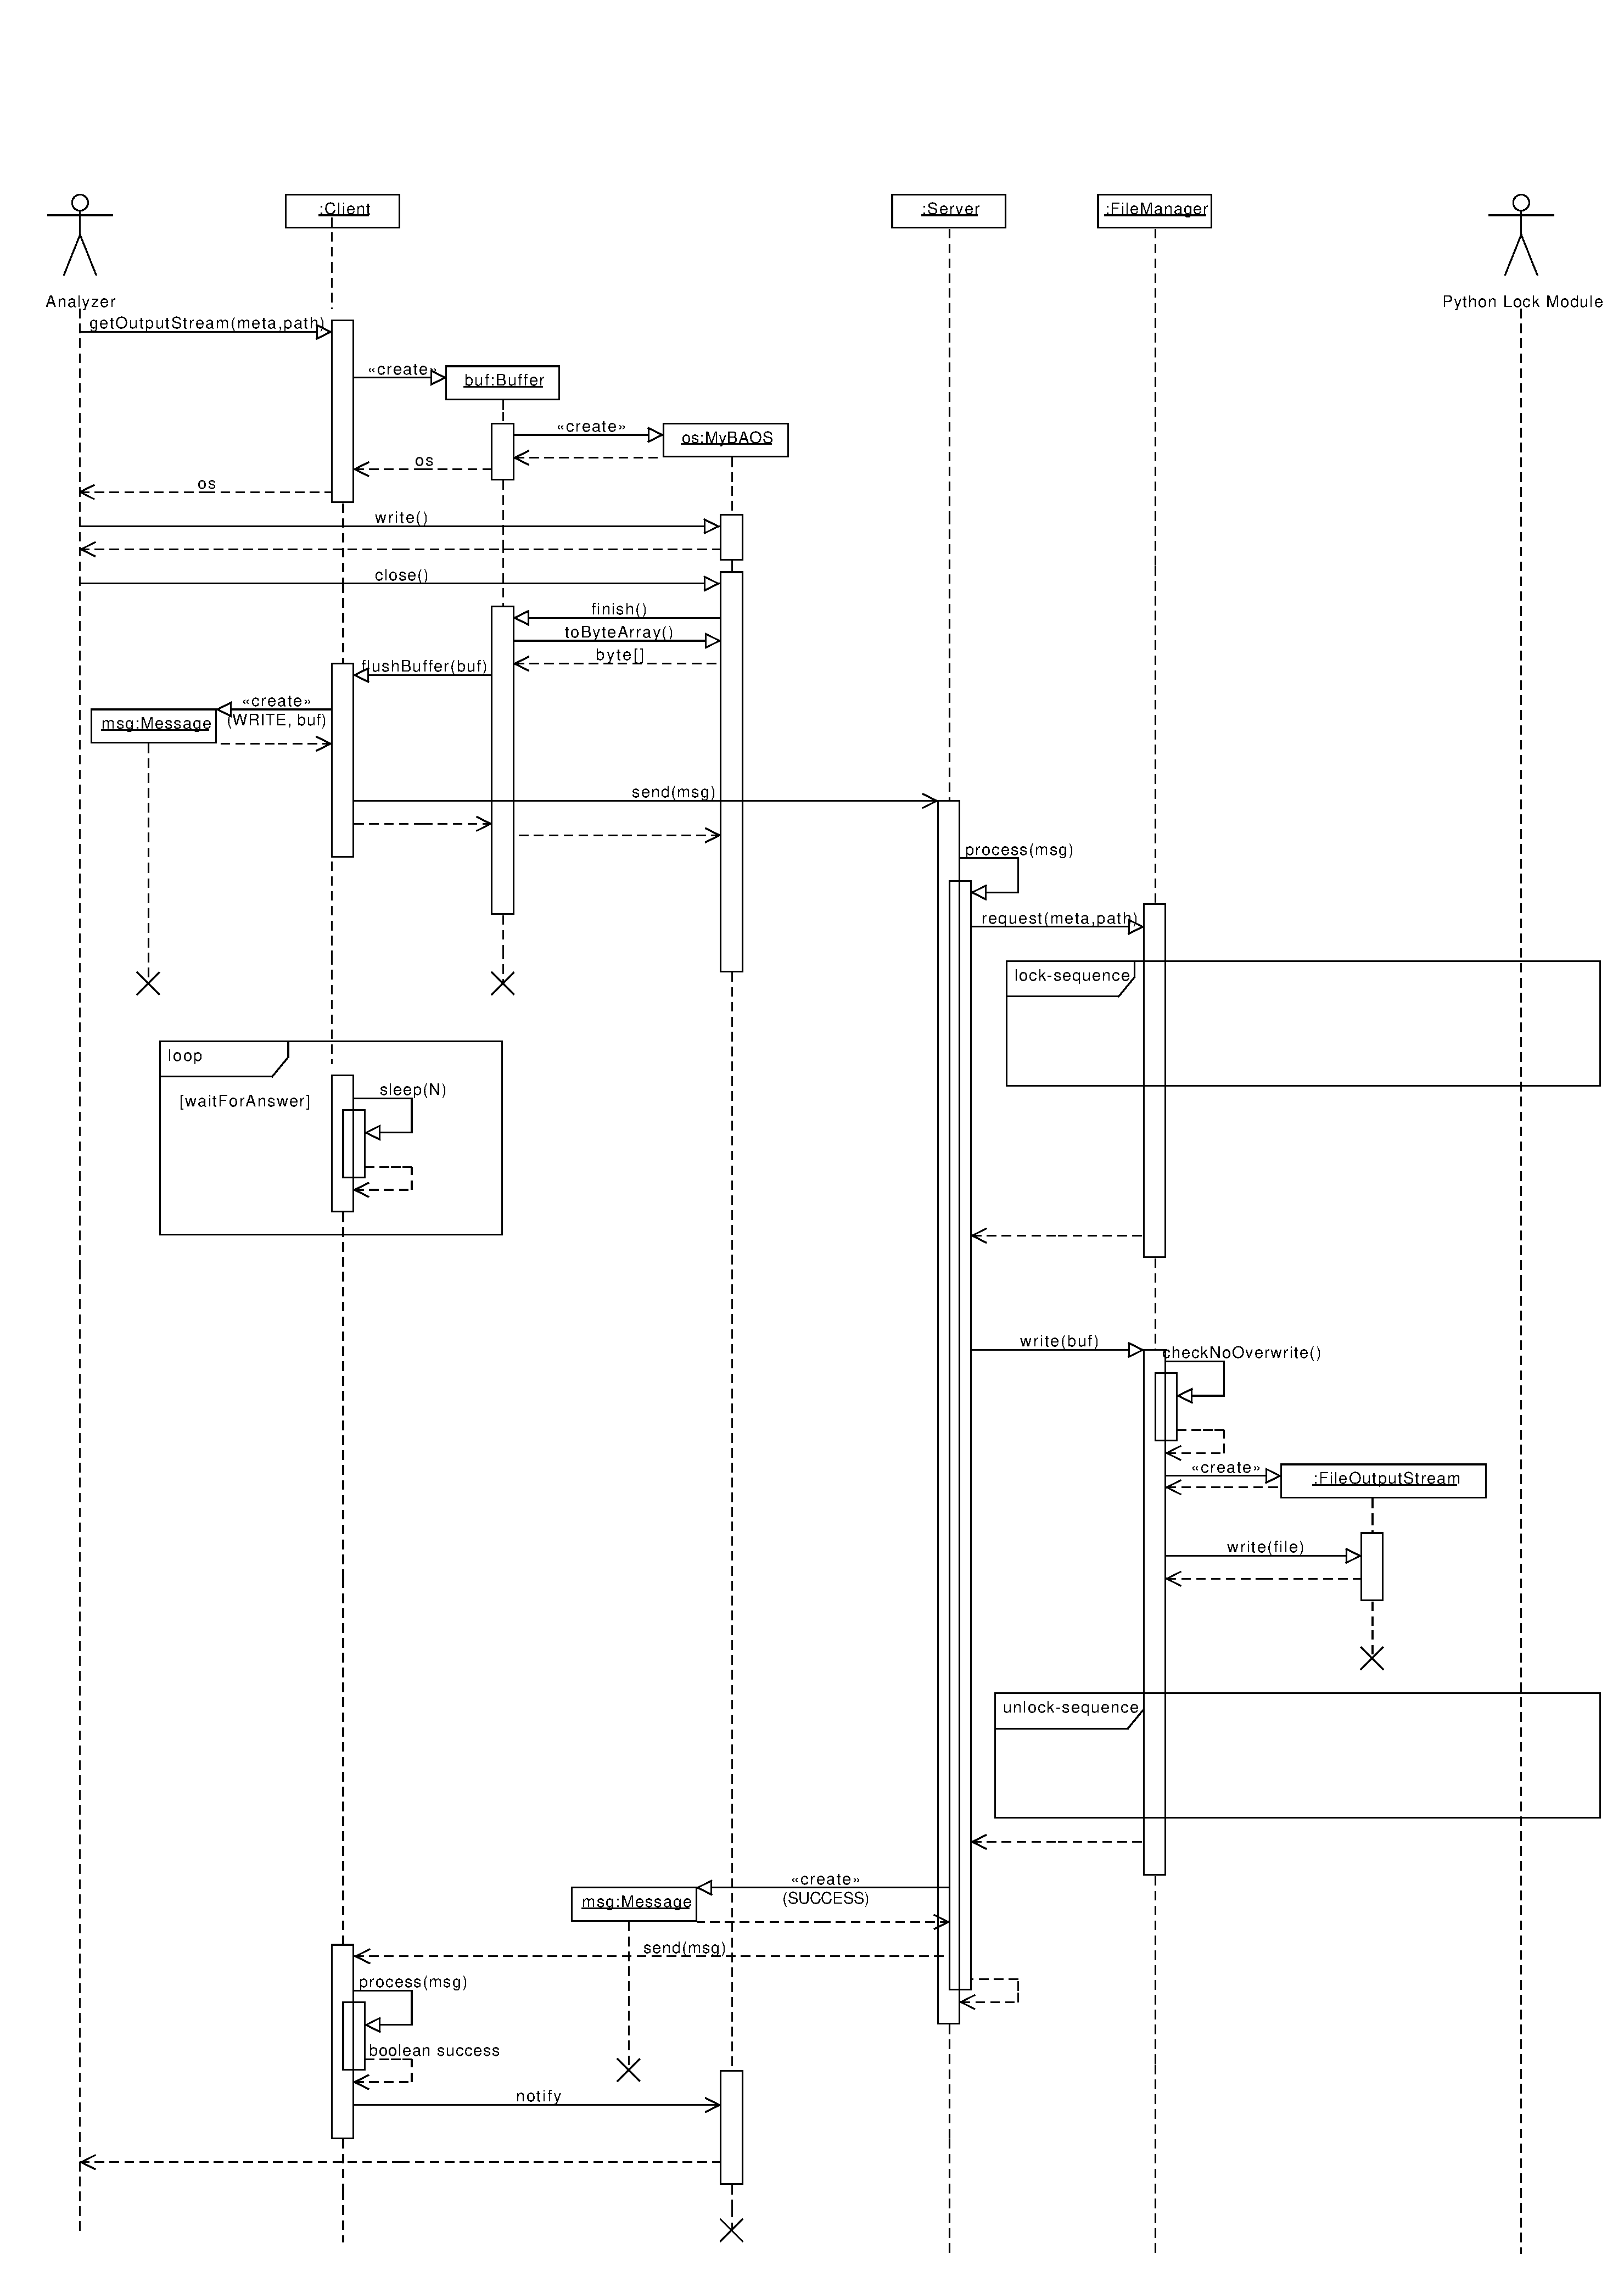
\includegraphics[width=\textwidth]{design/frontend/sequence/get-output-stream-sequence.pdf}
	\caption{Sequenzdiagramm: getOutputStream}
\end{figure}

\subsection {getInputStream}
\begin{figure}[!h]
	\centering
	\label{dia:design:frontend:sqc:getInputStream}
	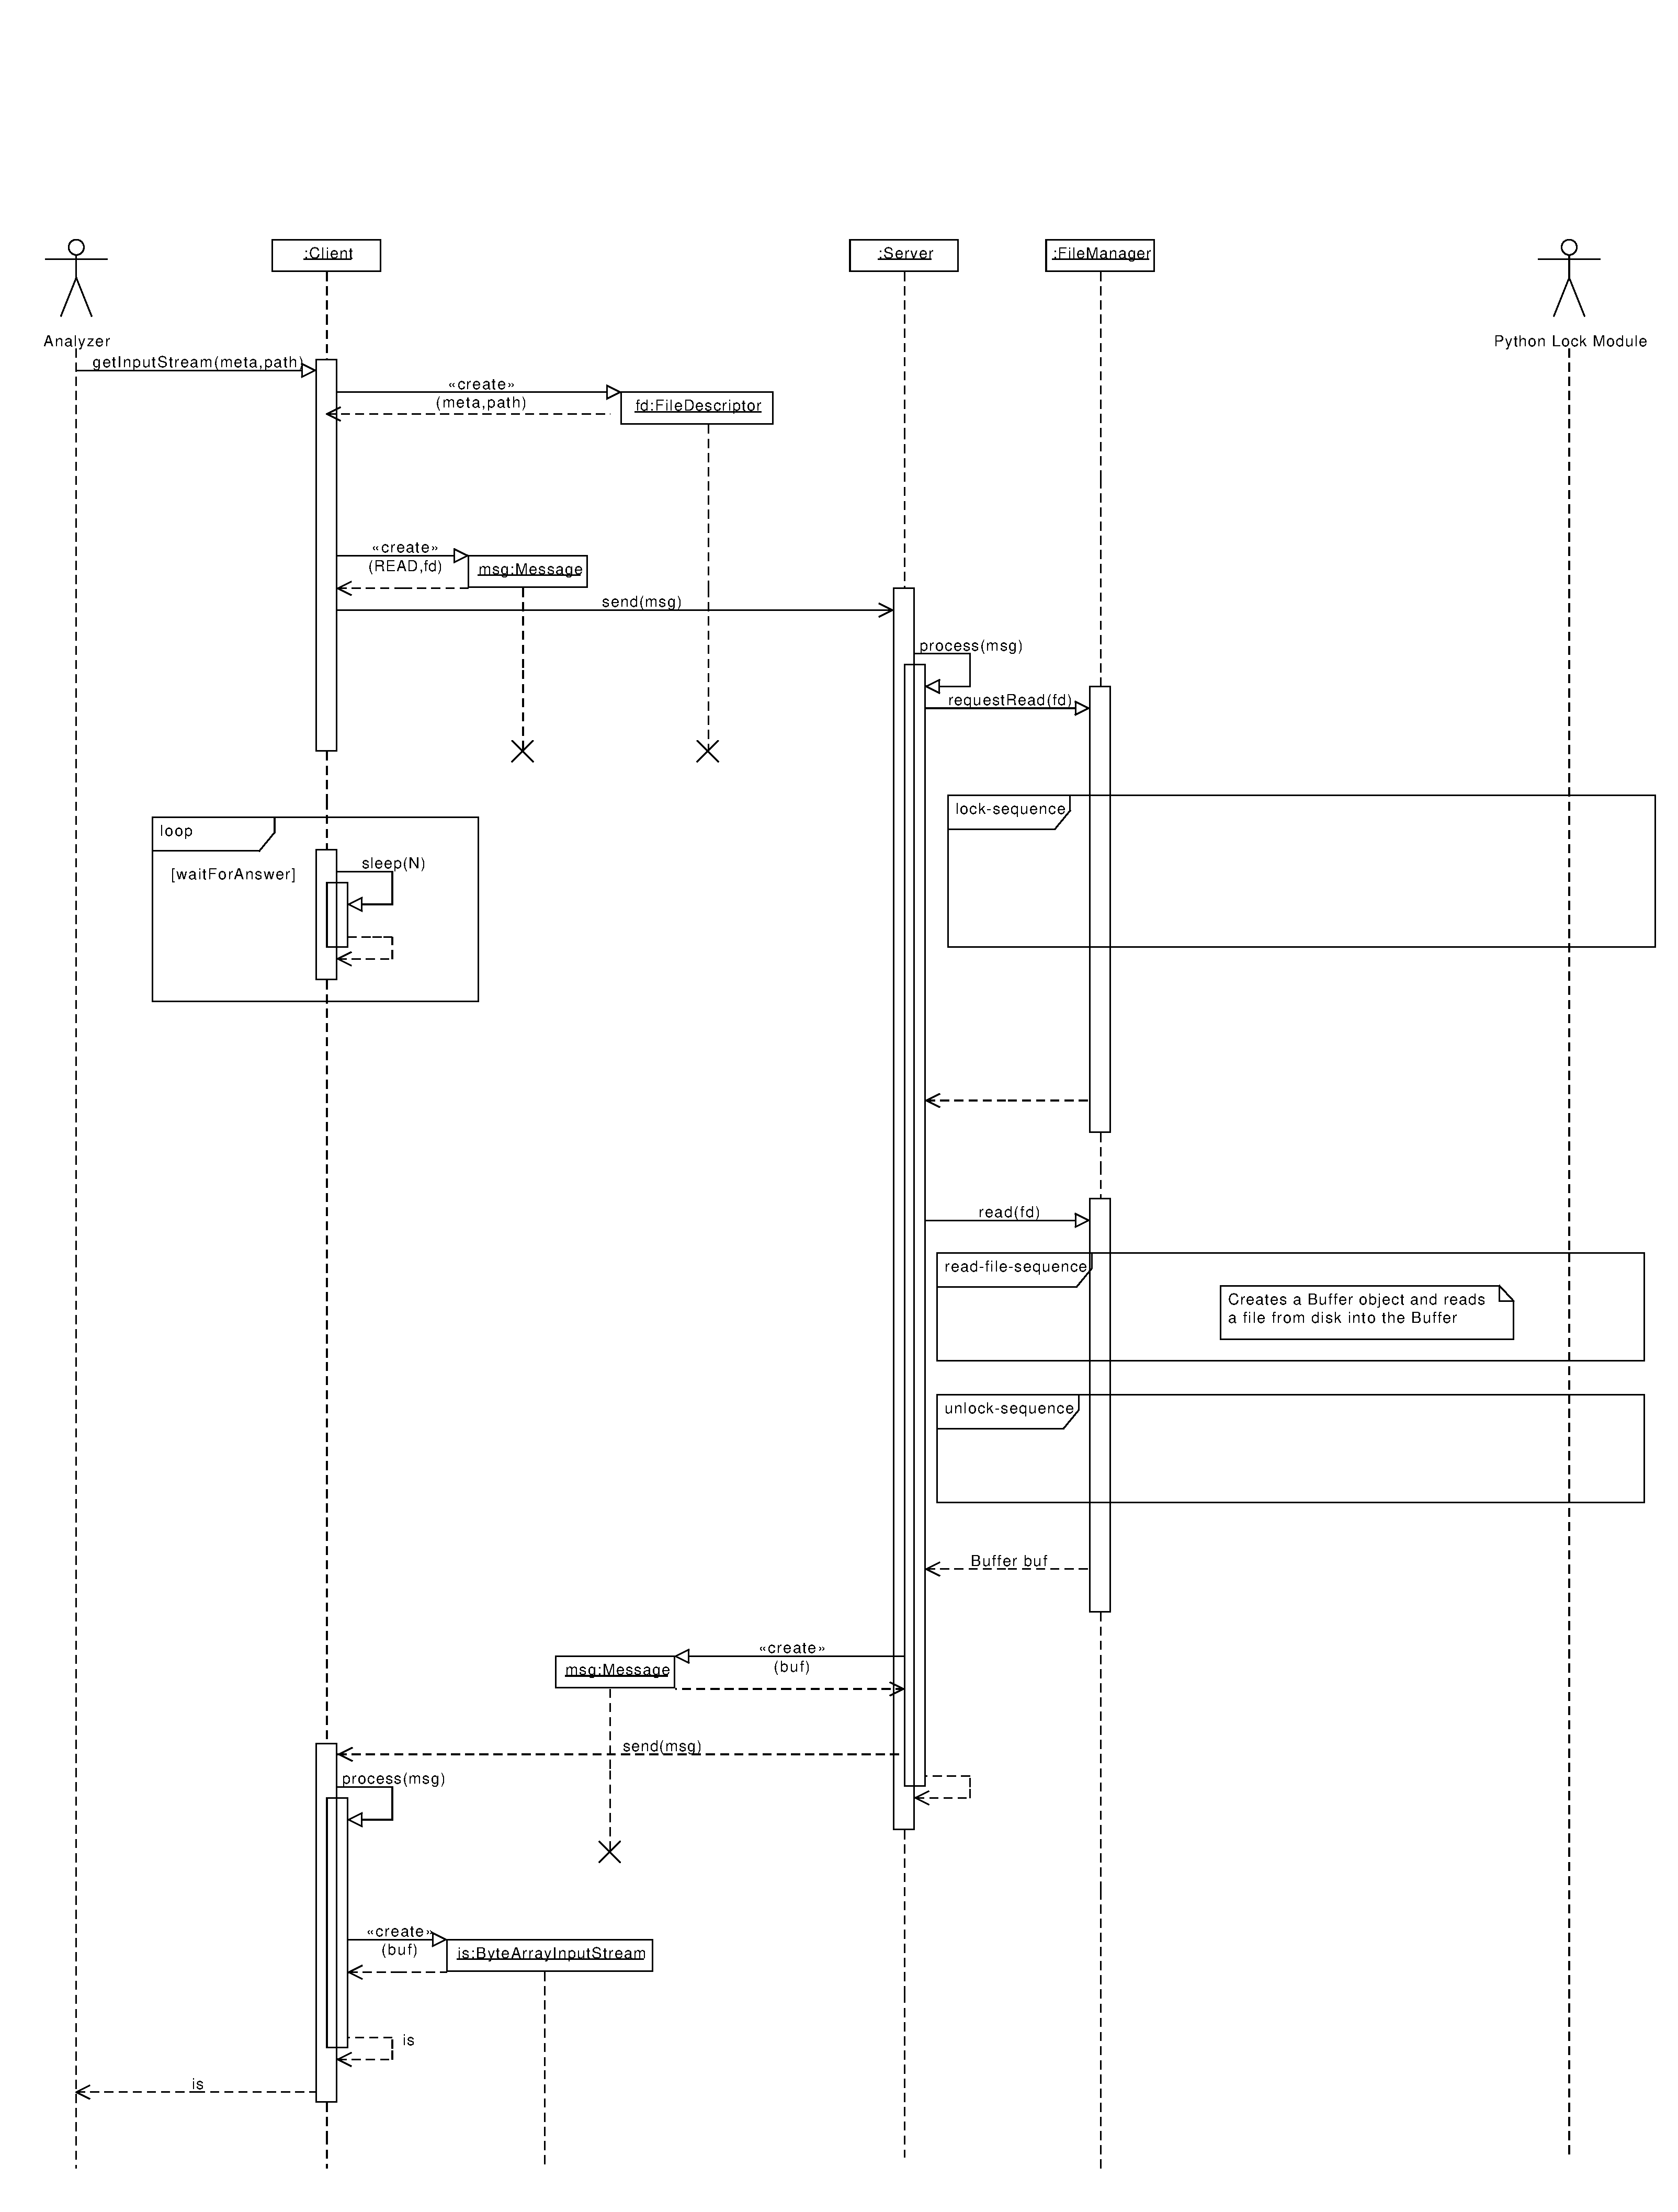
\includegraphics[width=0.5\textwidth]{design/frontend/sequence/get-input-stream-sequence.pdf}
	\caption{Sequenzdiagramm: getInputStream}
\end{figure}

\subsection {getXMLData}
\todo{sequence: getXMLData}
%\begin{figure}[h]
%	\centering
%	\label{dia:design:frontend:sqc:select}
%	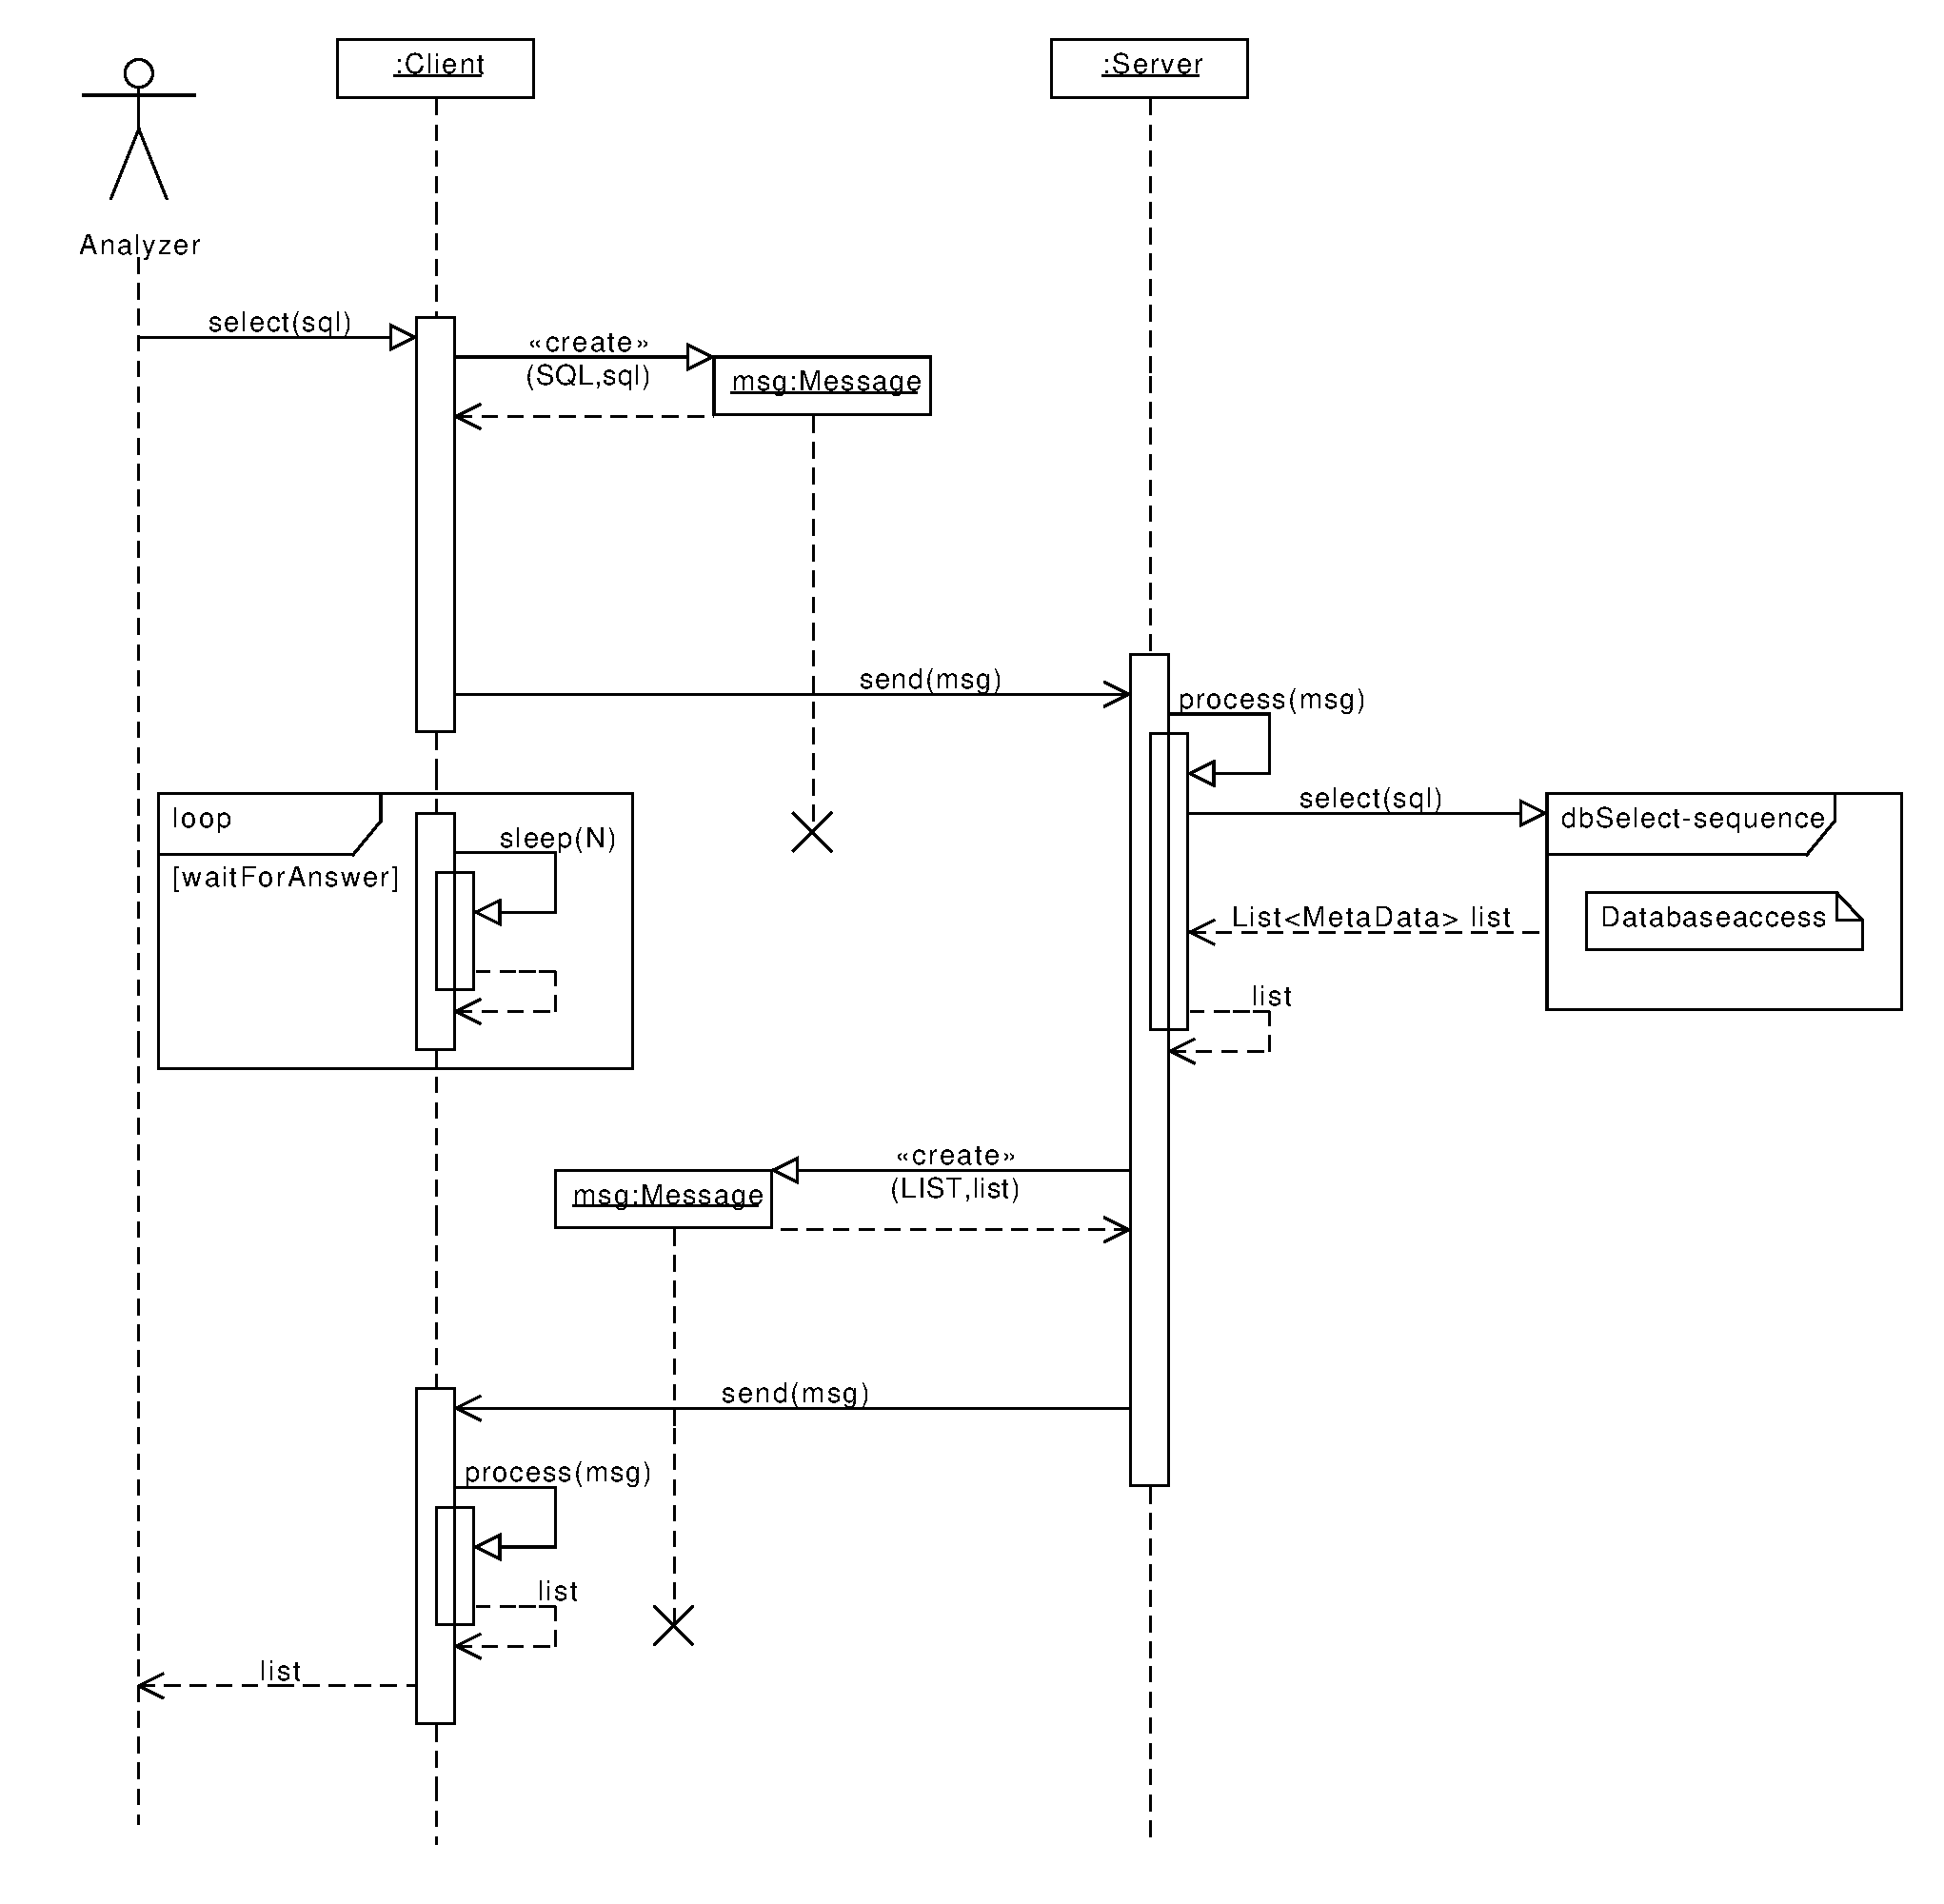
\includegraphics[width=\textwidth]{design/frontend/sequence/select-sequence.pdf}
%	\caption{Sequenzdiagramm: Select}
%\end{figure}

\subsection {addXMLData}
\todo{sequence: addXMLData}
%\begin{figure}[h]
%	\centering
%	\label{dia:design:frontend:sqc:select}
%	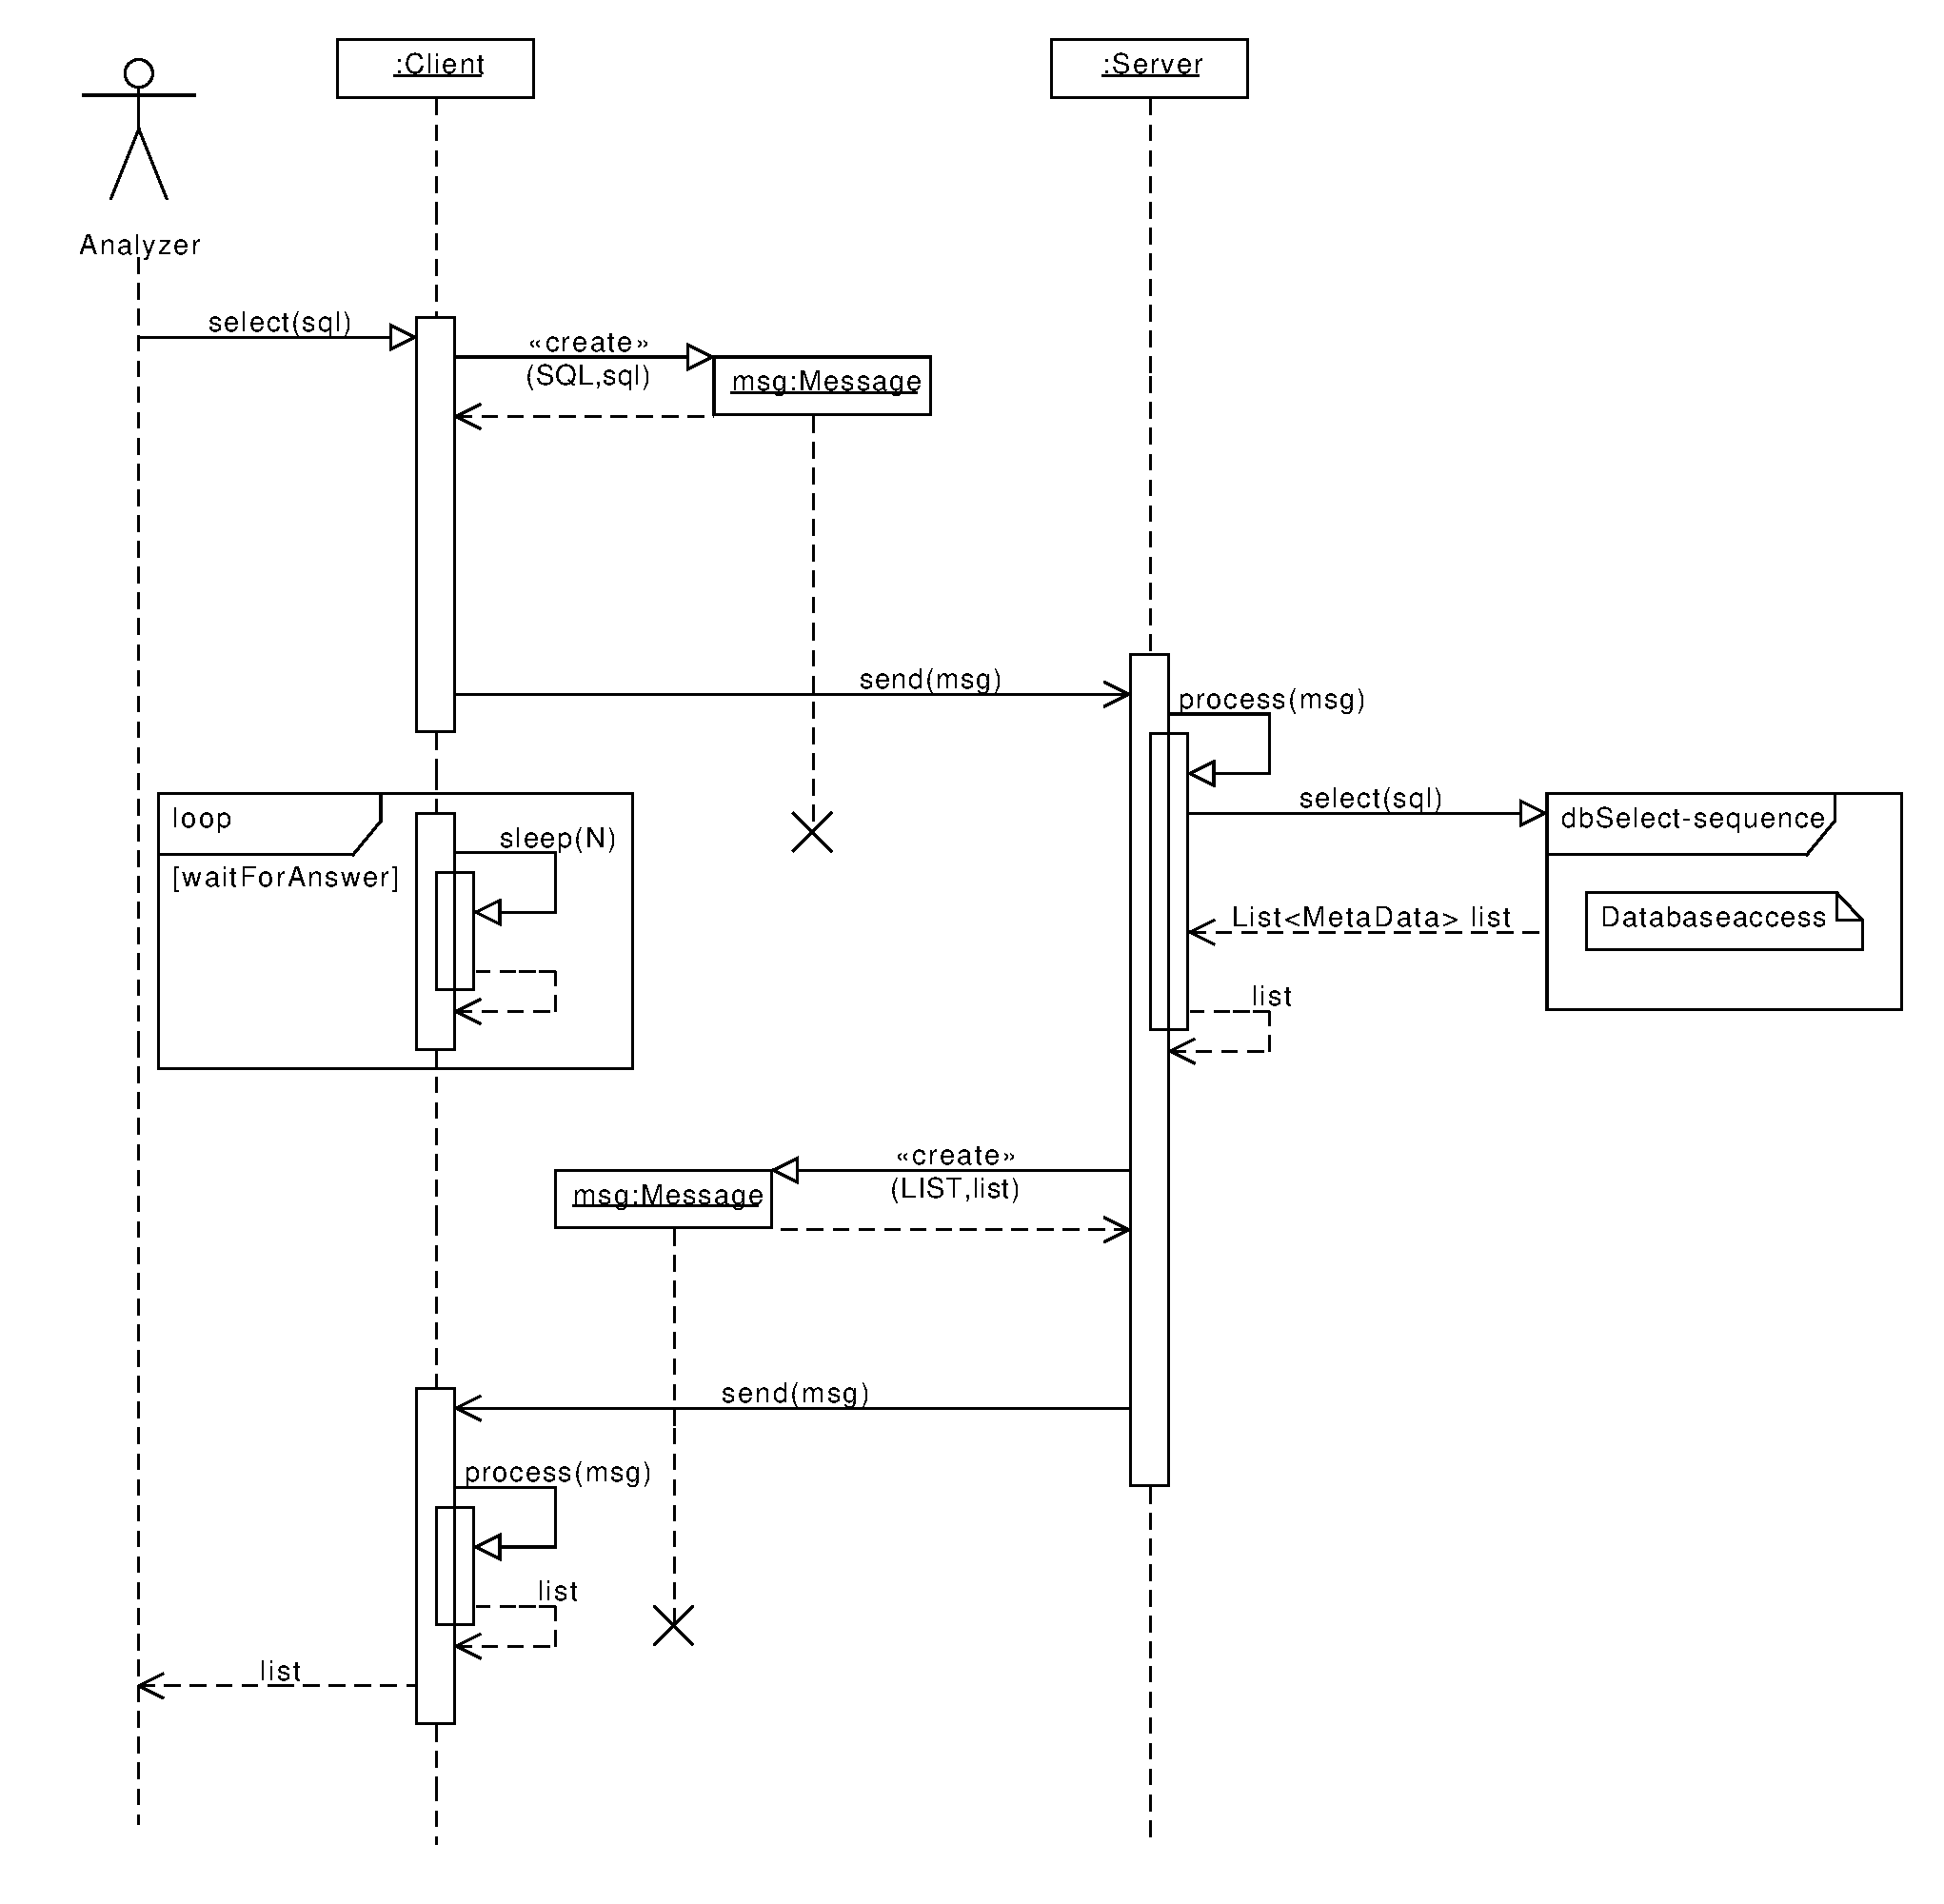
\includegraphics[width=\textwidth]{design/frontend/sequence/select-sequence.pdf}
%	\caption{Sequenzdiagramm: Select}
%\end{figure}

\subsection {add / deleteObserver}
\todo{sequence: addObserver}
%\begin{figure}[h]
%	\centering
%	\label{dia:design:frontend:sqc:select}
%	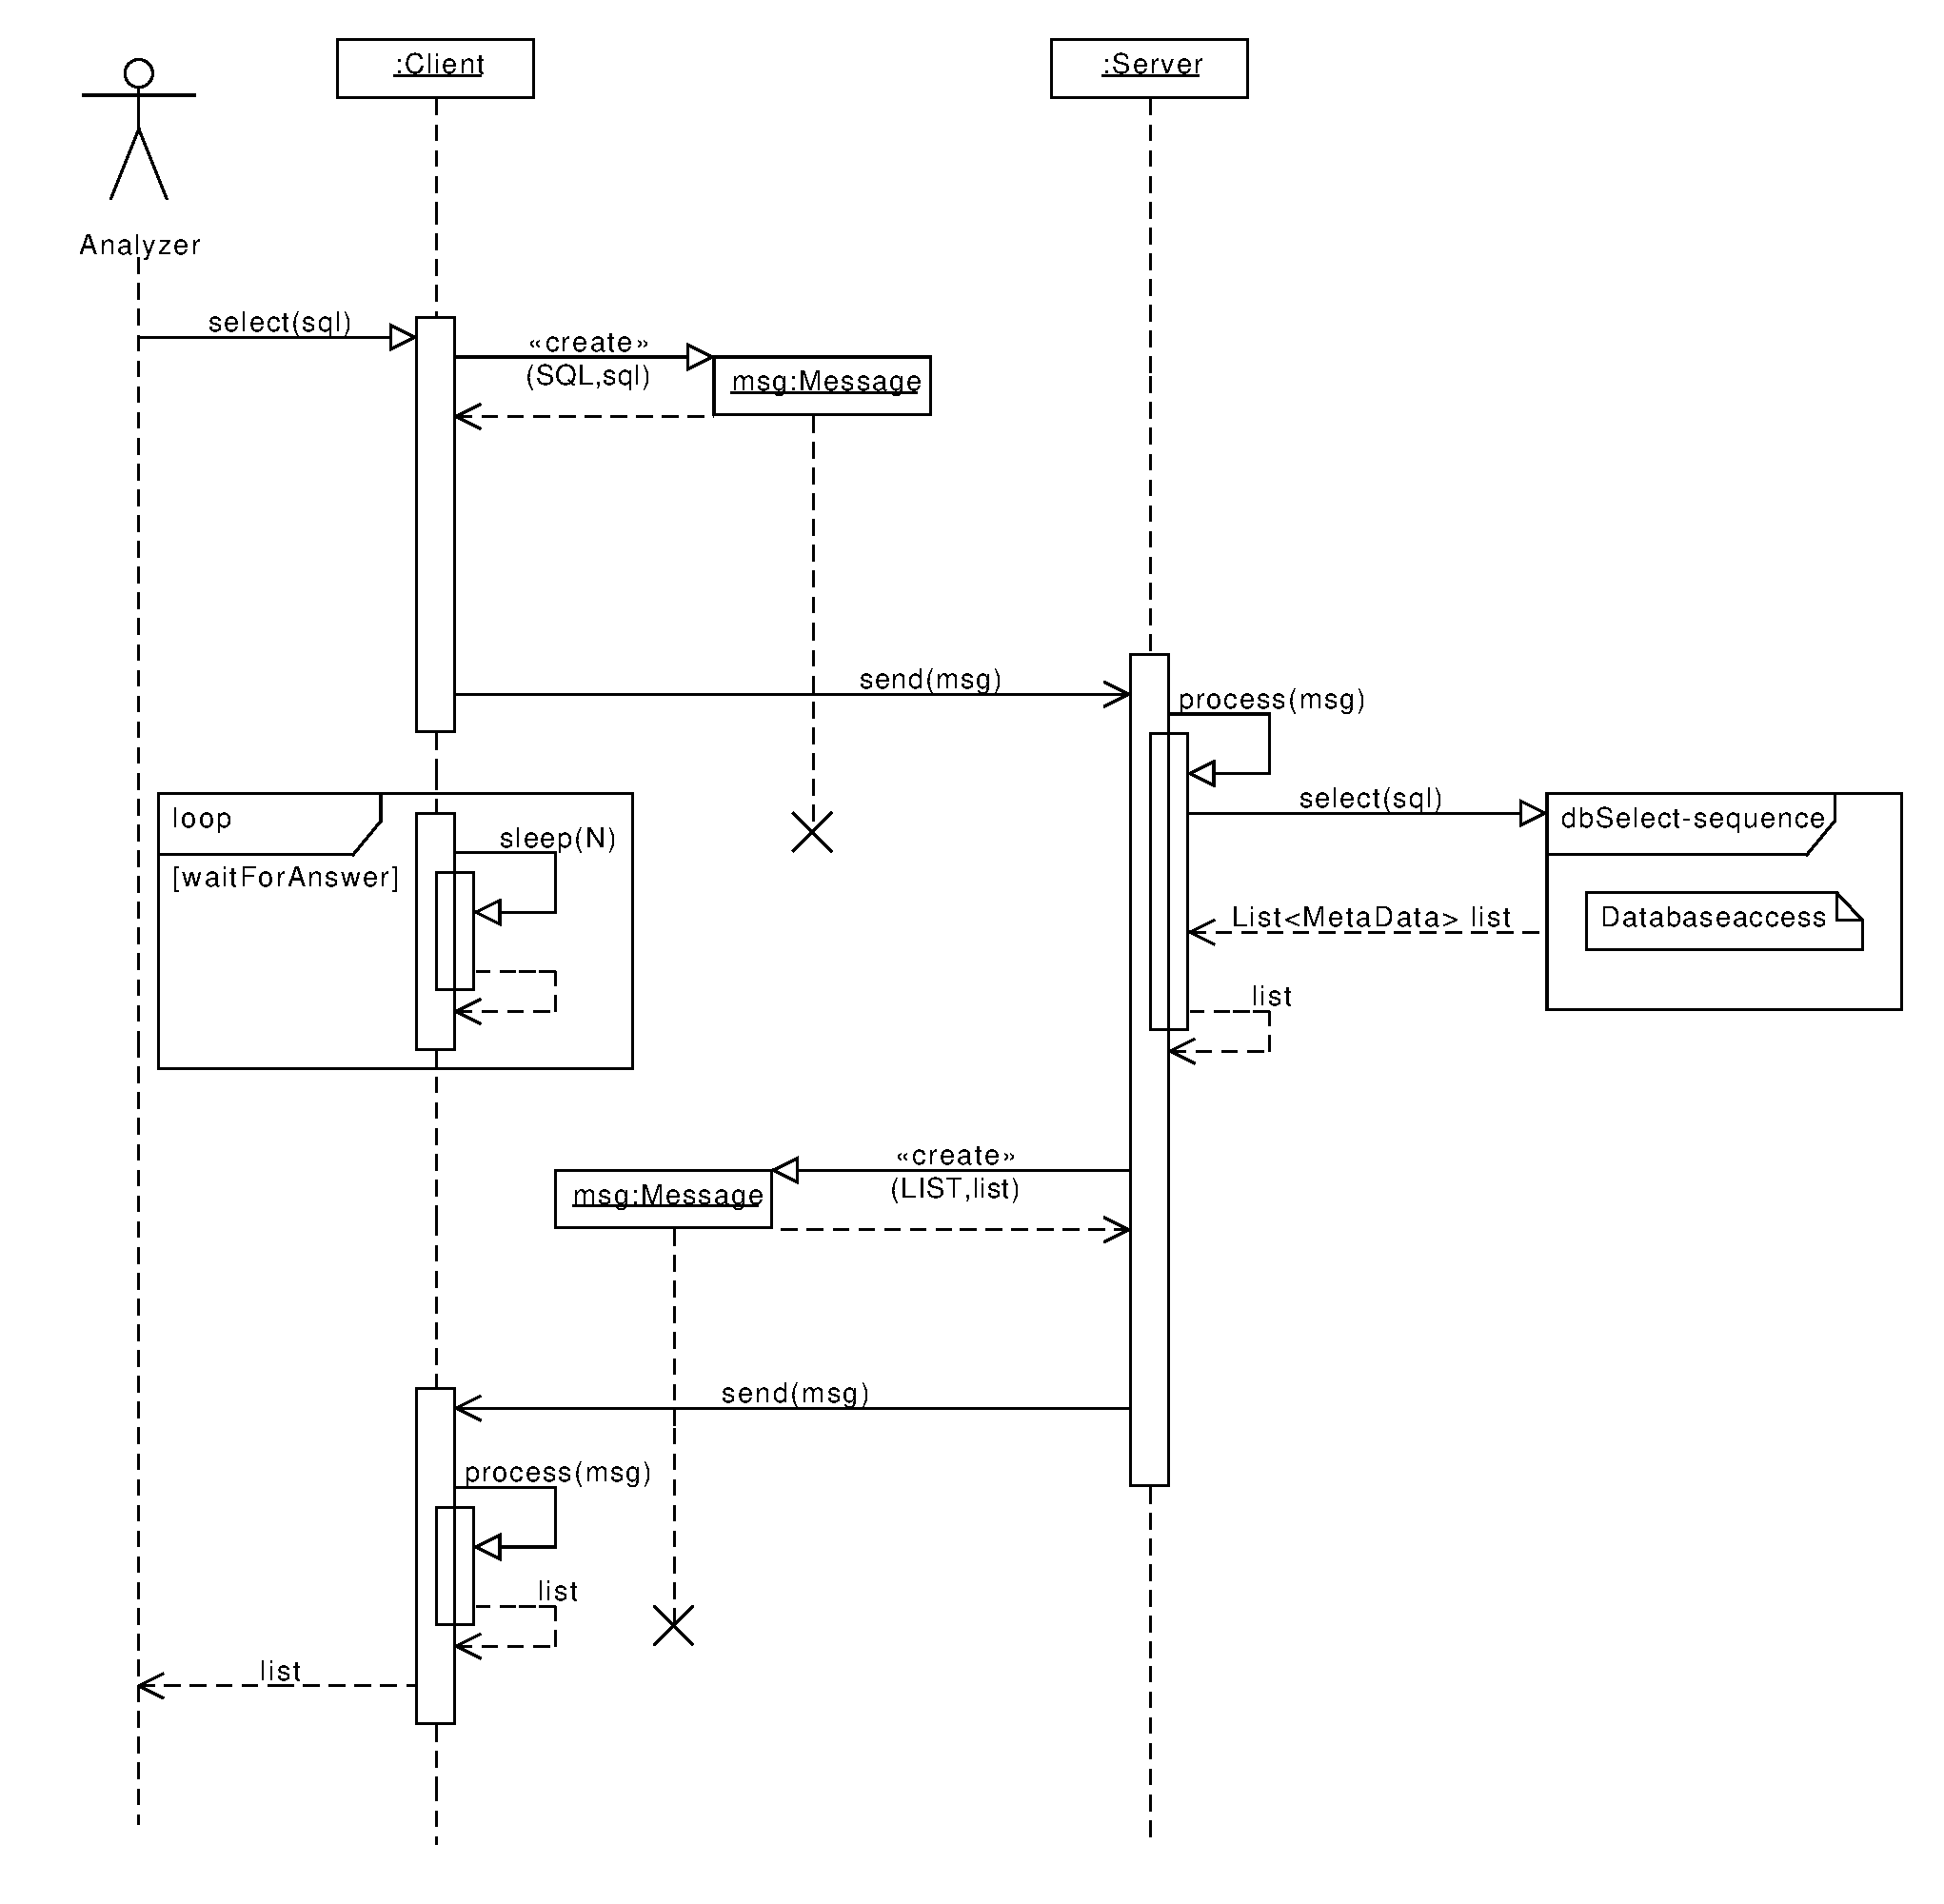
\includegraphics[width=\textwidth]{design/frontend/sequence/select-sequence.pdf}
%	\caption{Sequenzdiagramm: Select}
%\end{figure}

\subsection {notifyClients}
\todo{sequence: notifyClients}
%\begin{figure}[h]
%	\centering
%	\label{dia:design:frontend:sqc:select}
%	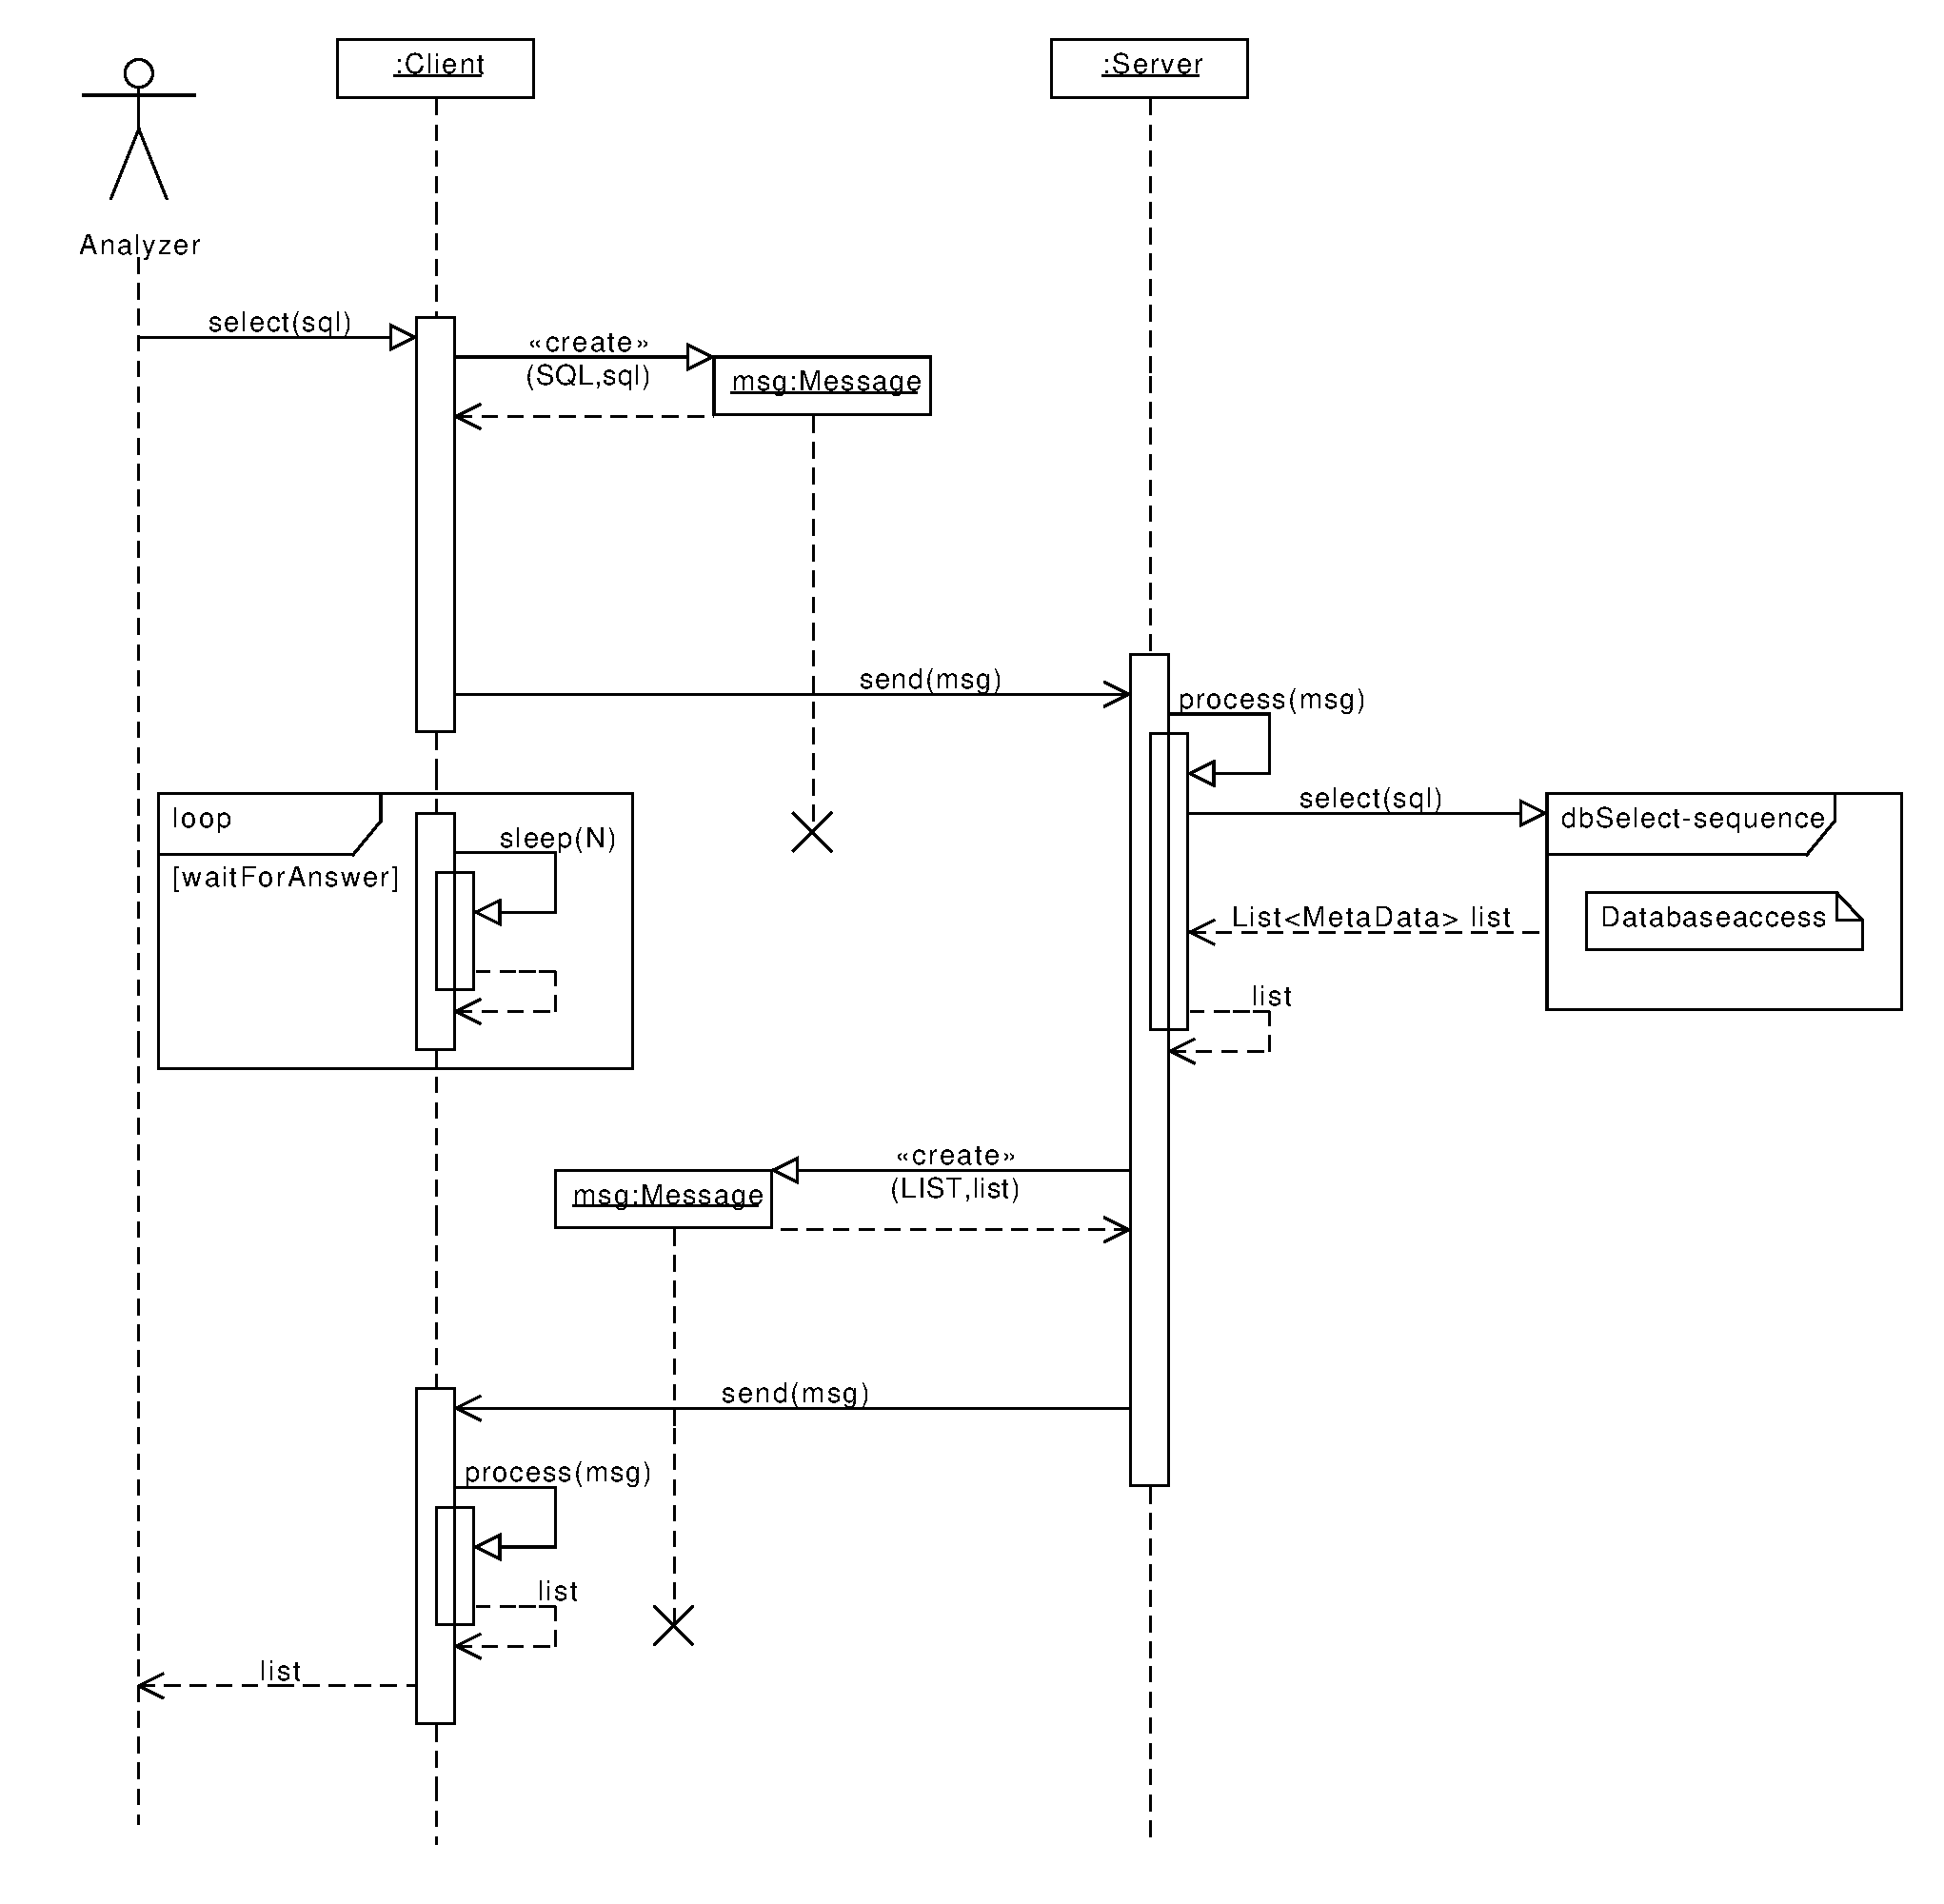
\includegraphics[width=\textwidth]{design/frontend/sequence/select-sequence.pdf}
%	\caption{Sequenzdiagramm: Select}
%\end{figure}

\subsection {Exception Handling}
\ref{req:Sv:comm:exceptions}
\section{Klassen und Komponenten}
\ref{req:Sv:comm}
\section{Test Analysetool} \ref{req:Cl:testanalyzer}
